\documentclass[11pt,a4paper]{article}
\usepackage[utf8]{inputenc}
\usepackage[T1]{fontenc}
\usepackage[lithuanian]{babel}
\usepackage{amsmath, amssymb}
\usepackage{tikz}
\usepackage{geometry}
\geometry{top=2cm, bottom=2cm, left=2cm, right=2cm}
\usepackage{parskip}

\begin{document}

\section*{Užduotys}

\noindent\textbf{I dalis}

\begin{enumerate}
    \item Taškų $A$ ir $B$ atstumai nuo horizontalios tiesės $l$ yra atitinkamai lygūs $3\text{ cm}$ ir $5\text{ cm}$. Atstumas tarp taško $A$ ir taško $B$ projekcijų tiesėje $l$ yra lygus $10\text{ cm}$. Tarkime, kad taškas $P$ yra bet kuris tiesės $l$ taškas. Raskite pačią mažiausią galimą $AP + PB$ reikšmę.
    
    \begin{center}
    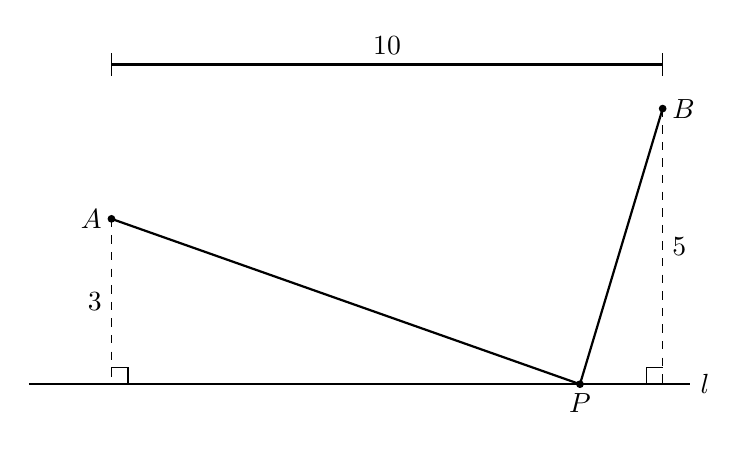
\begin{tikzpicture}[scale=0.7]
        % Tiesė l
        \draw[thick] (-0.5, 0) -- (11.5, 0) node[right] {$l$};
        
        % Taškai
        \coordinate (A) at (1, 3);
        \coordinate (B) at (11, 5);
        \coordinate (A0) at (1, 0);
        \coordinate (B0) at (11, 0);
        \coordinate (P) at (9.5, 0);
        
        % Statmenys į tiesę l
        \draw[dashed] (A) -- (A0);
        \draw[dashed] (B) -- (B0);
        
        % Lūžtanti linija APB
        \draw[thick] (A) -- (P) -- (B);
        
        % Taškų žymėjimas
        \fill (A) circle (2pt) node[left] {$A$};
        \fill (B) circle (2pt) node[right] {$B$};
        \fill (P) circle (2pt) node[below] {$P$};
        
        % Statumo kampai
        \draw (A0) ++(0, 0.3) -- ++(0.3, 0) -- ++(0, -0.3);
        \draw (B0) ++(0, 0.3) -- ++(-0.3, 0) -- ++(0, -0.3);
        
        % Matmenų žymėjimas
        \node[left] at (1, 1.5) {$3$};
        \node[right] at (11, 2.5) {$5$};
        
        % Viršutinė matmenų rodyklė / atkarpa
        \draw[thick] (1, 5.8) -- (11, 5.8);
        \draw (1, 5.6) -- (1, 6.0);
        \draw (11, 5.6) -- (11, 6.0);
        \node[above] at (6, 5.8) {$10$};
    \end{tikzpicture}
    \end{center}

    \item Kiek yra skirtingų natūraliųjų skaičių $a$ ir $b$ porų ($a \le 1\,000\,000$, $b \le 1\,000\,000$), su kuriomis būtų teisinga lygybė
    \[
    \frac{a^3 - b}{a^3 + b} = \frac{b^2 - a^2}{b^2 + a^2}\;?
    \]

    \item Apskaičiuokite reiškinio $x + \dfrac{1}{x}$ reikšmę, jeigu
    \[
    \frac{x^2 + x + 1}{x^2 - x + 1} = \frac{3}{2}.
    \]

    \item Skaičių seka $x_n$ yra apibrėžta tokiu būdu: $x_1 = 1$, $x_{n+1} = \dfrac{x_n}{n \cdot x_n + 1}$, $n \ge 1$. Raskite $x_{101}$.

    \item Visi natūralieji skaičiai surašyti didėjimo tvarka. Kiekvieną iš jų reikia nuspalvinti geltona, žalia arba raudona spalvomis. Jeigu skaičius geltonas, tai jo šeštasis kaimynas iš dešinės turi būti žalias; jeigu skaičius žalias, tai jo šeštasis kaimynas iš dešinės turi būti raudonas; jeigu skaičius raudonas, tai jo šeštasis kaimynas iš dešinės turi būti geltonas. Kiek yra skirtingų būdų tai padaryti?

    \item Skaitmenys $a$ ir $b$ yra tokie, kad $1 < a < b < 8$. Aštuonių mažiausių keturženklių skaičių, sudarytų iš skaitmenų $1, a, b, 8$ (skaitmenys skaičiuje gali būti panaudoti ne visi, t.\,y. gali kartotis), suma yra lygi $8994$. Raskite $a + b$.

    \item Profesorius Matemateriksas turi irklinę valtį. Vieną dieną jis nusprendė leistis į kelionę vietine upe. Pirmiausiai, profesorius plaukė 8 valandas prieš srovę, kol pasiekė poilsio vietą. Vėliau, kiek pailsėjęs, profesorius išplaukė namo. Lygiai po 4 valandų irklavimo jį išgąsdino garsus paukščio klyksmas ir Matemateriksas paleido iš rankų irklus, o šie įkrito į vandenį ir nuplaukė pasroviui. Likusį kelią iki namų valtį nešė srovė. Nepaisant to, profesoriui sugrįžti atgal užtruko 2 valandomis trumpiau, nei nuplaukti iki poilsio vietos. Apskaičiuokite upės tėkmės greitį (km/h), jeigu žinoma, kad stovinčiame vandenyje profesorius irkluoja pastoviu $7\text{ km/h}$ greičiu.

    \item Lentoje yra užrašyti du skirtingi dviženkliai skaičiai. Rokas juos sudaugino ir gavo keturženklį skaičių, kurio pirmasis skaitmuo lygus 2. Paulina lentoje užrašytus skaičius sudėjo ir gavo triženklį skaičių. Jeigu išbrauktume Roko gauto skaičiaus pirmąjį skaitmenį, tai likęs skaičius būtų 24 didesnis už Paulinos gautą skaičių. Raskite visas galimas dviženklių skaičių poras, kurios galėjo būti užrašytos lentoje. Laikykite, kad pirmasis poros skaičius yra mažesnis už antrąjį.

    \item Raskite keturženklį skaičių, sudarytą tik iš skaitmenų 1 ir 2, kuris dalinasi iš 16 be liekanos.

    \item Ignas šaškių turnyre sužaidė 52 partijas. Jeigu teisėjas už pergalę skirtų 1 tašką, už lygiąsias skirtų 0,5 taško, o už pralaimėjimą --- 0 taškų, tai Ignas surinktų 35 taškus. Kiek taškų pelnytų Ignas, jeigu pergalė būtų vertinama 1 tašku, lygiosios --- 0 taškų, o už pralaimėjimą būtų skirtas -1 taškas?
\end{enumerate}

\vspace{3mm}
\noindent\textbf{II dalis}

\begin{enumerate}
    \item Į kvadratą, kurio kraštinės ilgis lygus 1, yra įbrėžta ketvirtis vieno ir pusė kito apskritimo lanko (kaip parodyta brėžinyje). Mažiausias apskritimas liečia abiejų apskritimų dalių lankus bei kvadrato kraštinę. Raskite mažiausiojo apskritimo spindulį.
    
    \item Keliais skirtingais būdais skaičių $1\,000\,000$ galima išreikšti trijų natūraliųjų daugiklių sandauga, jeigu: \\
    a) į daugiklių tvarką atsižvelgiama? \\
    b) į daugiklių tvarką neatsižvelgiama?
\end{enumerate}

\vspace{2mm}
\noindent\textbf{Taškų suma:} \dotfill

\vspace{3mm}
\noindent\textit{\footnotesize Pastaba: Antrosios dalies sprendimai taisomi tik tada, kai pirmoje dalyje surinkta 7 ir daugiau taškų.}

\newpage
\section*{Atsakymai}

\subsection*{I dalis}
\begin{enumerate}
    \item $2\sqrt{41}$
    \item $15$
    \item $5$
    \item $\frac{1}{5051}$
    \item $729$
    \item $8$
    \item $2$
    \item $(26, 82)$ ir $(28, 76)$
    \item $2112$
    \item $18$
\end{enumerate}

\subsection*{II dalis}
\begin{enumerate}
    \item $\frac{3-2\sqrt{2}}{2}$
    \item a) $784$; \quad b) $139$
\end{enumerate}

\newpage
\section*{Sprendimai}

\subsection*{I dalis}
\begin{enumerate}
    \item \textbf{Sprendimas.}
    
    Norėdami rasti mažiausią atstumą $AP + PB$, pritaikysime atspindžio metodą. Tašką $A$ atspindime tiesės $l$ atžvilgiu ir gauname tašką $A'$. Atstumas nuo $A'$ iki tiesės $l$ taip pat yra 3.
    Dėl simetrijos bet kuriam tiesės $l$ taškui $P$ galioja lygybė $AP = A'P$. Tada mūsų ieškoma suma virsta:
    \[ AP + PB = A'P + PB. \]
    Ši suma bus mažiausia tada, kai taškai $A'$, $P$ ir $B$ gulės vienoje tiesėje (trumpiausias atstumas tarp dviejų taškų yra tiesės atkarpa). Vadinasi, ieškomas minimalus atstumas yra atkarpos $A'B$ ilgis.
    
    \begin{center}
    \begin{tikzpicture}[scale=0.7]
        % Tiesė l
        \draw[thick] (-1, 0) -- (11, 0) node[right] {$l$};
        
        % Taškai
        \coordinate (A) at (0, 3);
        \coordinate (A_proj) at (0, 0);
        \coordinate (A_ref) at (0, -3);
        \coordinate (B) at (10, 5);
        \coordinate (B_proj) at (10, 0);
        
        % Atspindys ir tiesė A'B
        \draw[dashed] (A) -- (A_ref);
        \draw[dashed] (B) -- (B_proj);
        \draw[thick, red] (A_ref) -- (B) coordinate[pos=0.375] (P);
        
        % Pradinės atkarpos AP ir PB
        \draw[thick, blue] (A) -- (P) -- (B);
        
        % Taškų žymėjimas
        \fill (A) circle (2pt) node[above left] {$A$};
        \fill (A_ref) circle (2pt) node[below left] {$A'$};
        \fill (B) circle (2pt) node[above right] {$B$};
        \fill (P) circle (2pt) node[above left] {$P$};
        
        % Matmenų žymėjimas
        \node[left] at (0, 1.5) {$3$};
        \node[left] at (0, -1.5) {$3$};
        \node[right] at (10, 2.5) {$5$};
        
        % 10 cm atstumas
        \draw[<->] (0, -0.5) -- (10, -0.5) node[midway, below] {$10$};
        
        % Statumo kampai
        \draw (A_proj) ++(0, 0.3) -- ++(0.3, 0) -- ++(0, -0.3);
        \draw (B_proj) ++(0, 0.3) -- ++(-0.3, 0) -- ++(0, -0.3);
    \end{tikzpicture}
    \end{center}
    
    Nagrinėjame statųjį trikampį, kurio horizontalus statinis lygus atstumui tarp projekcijų (10), o vertikalus statinis lygus $5 - (-3) = 8$. Pagal Pitagoro teoremą atkarpos $A'B$ ilgis:
    \[ A'B = \sqrt{10^2 + 8^2} = \sqrt{100 + 64} = \sqrt{164} = 2\sqrt{41}. \]
    
    \textbf{Atsakymas:} $2\sqrt{41}$.

    \vspace{0.3cm}
    \item \textbf{Sprendimas.}
    
    Išsprendžiame duotą lygtį taikydami proporcijos savybę (dauginame kryžmai):
    \[ (a^3 - b)(b^2 + a^2) = (b^2 - a^2)(a^3 + b). \]
    Atskliaudžiame abi puses:
    \[ a^3b^2 + a^5 - b^3 - a^2b = a^3b^2 + b^3 - a^5 - a^2b. \]
    Suprastinę vienodus narius ($a^3b^2$ ir $-a^2b$) abiejose pusėse, gauname:
    \[ a^5 - b^3 = b^3 - a^5 \implies 2a^5 = 2b^3 \implies a^5 = b^3. \]
    Kadangi $a$ ir $b$ yra natūralieji skaičiai, o 5 ir 3 yra tarpusavyje pirminiai, abu skaičiai $a$ ir $b$ privalo būti to paties skaičiaus $x$ laipsniai, t.\,y., $a = x^3$ ir $b = x^5$, kur $x \in \mathbb{N}$.
    Pagal sąlygą $a \le 1\,000\,000$ ir $b \le 1\,000\,000$.
    \begin{itemize}
        \item $x^3 \le 1\,000\,000 \implies x \le 100$.
        \item $x^5 \le 1\,000\,000$. Kadangi $15^5 = 759\,375$, o $16^5 = 1\,048\,576$, tai $x \le 15$.
    \end{itemize}
    Kadangi turi būti tenkinamos abi sąlygos, $x$ gali įgyti bet kokią natūraliąją reikšmę nuo 1 iki 15 imtinai. Tokių $x$ reikšmių, o kartu ir $(a, b)$ porų, yra 15.
    
    \textbf{Atsakymas:} $15$.

    \vspace{0.3cm}
    \item \textbf{Sprendimas.}
    
    Duota lygtis:
    \[ \frac{x^2 + x + 1}{x^2 - x + 1} = \frac{3}{2}. \]
    Padaliname skaitiklį ir vardiklį iš $x$ (pastebime, kad $x \neq 0$):
    \[ \frac{x + 1 + \frac{1}{x}}{x - 1 + \frac{1}{x}} = \frac{3}{2}. \]
    Pažymėkime $y = x + \frac{1}{x}$. Tada lygtis atrodo taip:
    \[ \frac{y + 1}{y - 1} = \frac{3}{2}. \]
    Sprendžiame proporciją:
    \[ 2(y + 1) = 3(y - 1) \implies 2y + 2 = 3y - 3 \implies y = 5. \]
    Grįžę prie pažymėjimo, gauname: $x + \frac{1}{x} = 5$.
    
    \textbf{Atsakymas:} $5$.

    \vspace{0.3cm}
    \item \textbf{Sprendimas.}
    
    Duota rekurentinė formulė:
    \[ x_{n+1} = \frac{x_n}{n \cdot x_n + 1}. \]
    Apverskime abi lygties puses (imkime atvirkštinius dydžius):
    \[ \frac{1}{x_{n+1}} = \frac{n \cdot x_n + 1}{x_n} = n + \frac{1}{x_n}. \]
    Pažymėkime seką $y_n = \frac{1}{x_n}$. Kadangi $x_1 = 1$, tai $y_1 = 1$. Tuomet gauname aritmetinę rekursiją:
    \[ y_{n+1} = y_n + n. \]
    Išrašykime kelis pirmuosius sekos narius:
    \begin{align*}
        y_2 &= y_1 + 1, \\
        y_3 &= y_2 + 2 = y_1 + 1 + 2, \\
        y_4 &= y_3 + 3 = y_1 + 1 + 2 + 3, \\
        \dots \\
        y_n &= y_1 + (1 + 2 + \dots + n - 1).
    \end{align*}
    Skliaustuose yra aritmetinės progresijos suma, lygi $\frac{(n-1)n}{2}$. Tuomet:
    \[ y_{101} = 1 + \frac{100 \cdot 101}{2} = 1 + 5050 = 5051. \]
    Kadangi ieškome $x_{101}$, grįžtame prie pradinio kintamojo:
    \[ x_{101} = \frac{1}{y_{101}} = \frac{1}{5051}. \]
    
    \textbf{Atsakymas:} $\frac{1}{5051}$.

    \vspace{0.3cm}
    \item \textbf{Sprendimas.}
    
    Pagal sąlygą kiekvieno skaičiaus $n+6$ spalva vienareikšmiškai priklauso nuo skaičiaus $n$ spalvos:
    \begin{itemize}
        \item Jei $n$ geltonas $\to n+6$ žalias.
        \item Jei $n$ žalias $\to n+6$ raudonas.
        \item Jei $n$ raudonas $\to n+6$ geltonas.
    \end{itemize}
    Tai reiškia, kad kai tik nudažome skaičius nuo 1 iki 6, visų likusių skaičių spalvos tampa automatiškai nulemtos (pvz., skaičiaus 7 spalvą lemia 1 spalva, skaičiaus 8 -- 2 spalva ir t.\,t.).
    Skaičiams nuo 1 iki 6 nudažyti jokių pradinių apribojimų nėra. Kiekvienam iš 6 skaičių galime rinktis iš 3 spalvų nepriklausomai vienas nuo kito. 
    Vadinasi, bendras skirtingų būdų skaičius yra:
    \[ 3 \cdot 3 \cdot 3 \cdot 3 \cdot 3 \cdot 3 = 3^6 = 729. \]
    
    \textbf{Atsakymas:} $729$.

    \vspace{0.3cm}
    \item \textbf{Sprendimas.}
    
    Turime skaitmenis $1, a, b, 8$, kur $1 < a < b < 8$. Sudarome aštuonis mažiausius keturženklius skaičius, kur skaitmenys gali kartotis. Mažiausi skaičiai visada prasidės pačiais mažiausiais įmanomais skaitmenimis, taigi visi 8 ieškomi skaičiai prasidės $11$.
    Jų išsidėstymas didėjimo tvarka, atsižvelgiant į sąlygą $1 < a < b < 8$:
    \[ 1111,\; 111a,\; 111b,\; 1118,\; 11a1,\; 11aa,\; 11ab,\; 11a8. \]
    Suskaičiuokime visų šių 8 skaičių sumą pagal skyrius:
    \begin{itemize}
        \item \textbf{Tūkstančiai ir šimtai:} $8 \cdot 1100 = 8800$.
        \item \textbf{Dešimtys:} turime keturis skaičius su dešimčių skaitmeniu 1 ir keturis su $a$. Jų suma: $(4 \cdot 1 + 4 \cdot a) \cdot 10 = 40 + 40a$.
        \item \textbf{Vienetai:} skaitmenų seka $(1, a, b, 8)$ vienetuose pasikartoja lygiai 2 kartus. Suma: $2 \cdot (1 + a + b + 8) = 18 + 2a + 2b$.
    \end{itemize}
    Sudedame visas dalis ir prilyginame 8994:
    \begin{align*}
        8800 + 40 + 40a + 18 + 2a + 2b &= 8994 \\
        8858 + 42a + 2b &= 8994 \\
        42a + 2b &= 136 \\
        21a + b &= 68.
    \end{align*}
    Išbandome galimas $a$ reikšmes, kai $1 < a < 8$:
    \begin{itemize}
        \item Jei $a = 2$, tai $42 + b = 68 \implies b = 26$ (netinka, nes $b < 8$).
        \item Jei $a = 3$, tai $63 + b = 68 \implies b = 5$.
    \end{itemize}
    Patikriname sąlygą $1 < a < b < 8 \implies 1 < 3 < 5 < 8$. Sąlyga tenkinama!
    Vadinasi $a = 3$, $b = 5$. Ieškoma suma:
    \[ a + b = 3 + 5 = 8. \]
    
    \textbf{Atsakymas:} $8$.

    \vspace{0.3cm}
    \item \textbf{Sprendimas.}
    
    Tegu upės tėkmės greitis yra $c$ (km/h). Stovinčiame vandenyje profesoriaus greitis $v = 7$ (km/h).
    Kelionė prieš srovę užtruko 8 valandas, taigi atstumas iki poilsio vietos yra:
    \[ s = 8(7 - c). \]
    Kelionė namo pasroviui:
    \begin{itemize}
        \item Profesorius 4 valandas irklavo pasroviui, todėl įveikė $4(7 + c)$ kilometrų.
        \item Likusį laiką valtį nešė tik upės srovė. Kadangi kelionė atgal užtruko 2 valandomis trumpiau nei pirmyn, vadinasi, ji truko $8 - 2 = 6$ valandas. Iš jų 4 valandos buvo irkluotos, tad srovė valtį nešė $6 - 4 = 2$ valandas. Nuplauktas atstumas: $2 \cdot c$.
    \end{itemize}
    Bendras atstumas grįžtant yra toks pat:
    \[ s = 4(7 + c) + 2c. \]
    Sulyginame abiejų kelionių atstumus:
    \begin{align*}
        8(7 - c) &= 4(7 + c) + 2c \\
        56 - 8c &= 28 + 4c + 2c \\
        28 &= 14c \implies c = 2\text{ km/h}.
    \end{align*}
    
    \textbf{Atsakymas:} $2$.

    \vspace{0.3cm}
    \item \textbf{Sprendimas.}
    
    Tegul lentoje užrašyti dviženkliai skaičiai yra $x$ ir $y$, kur $x < y$.
    Roko gautas keturženklis skaičius prasideda skaitmeniu 2, tad jį galime užrašyti kaip $2000 + R$, kur $R$ yra triženklis arba dviženklis skaičius ($R = x \cdot y - 2000$).
    Paulina gavo skaičių $x + y$.
    Išbraukus pirmąjį skaitmenį iš Roko rezultato, lieka skaičius $R$. Pagal sąlygą:
    \[ R = (x + y) + 24. \]
    Pakeičiame $R$ į $x \cdot y - 2000$:
    \begin{align*}
        x \cdot y - 2000 &= x + y + 24 \\
        x \cdot y - x - y &= 2024.
    \end{align*}
    Prie abiejų pusių pridėję po 1, išraišką galime išskaidyti dauginamaisiais:
    \[ (x - 1)(y - 1) = 2025. \]
    Ieškome skaičiaus 2025 daliklių $A$ ir $B$, kur $A \cdot B = 2025$. Kadangi $x$ ir $y$ yra skirtingi dviženkliai skaičiai, tai ir skaičiai $(x-1)$ bei $(y-1)$ turi būti skirtingi ir priklausyti intervalui nuo $10-1 = 9$ iki $99-1 = 98$.
    Išskaidykime $2025 = 25 \cdot 81 = 27 \cdot 75 = 45 \cdot 45$. 
    \begin{itemize}
        \item Jei $A = 25, B = 81$, tuomet $x = 26$ ir $y = 82$.
        \item Jei $A = 27, B = 75$, tuomet $x = 28$ ir $y = 76$.
        \item (Variantas $A=45, B=45$ netinka, nes skaičiai turi būti skirtingi).
    \end{itemize}
    Abi šios poros atitinka visas sąlygas.
    
    \textbf{Atsakymas:} $(26, 82)$ ir $(28, 76)$.

    \vspace{0.3cm}
    \item \textbf{Sprendimas.}
    
    Ieškome keturženklio skaičiaus, sudaryto iš 1 ir 2, daloraus iš 16. Skaičius dalijasi iš 16 tada ir tik tada, kai paskutinių jo 4 skaitmenų sudarytas skaičius dalijasi iš 16. Kadangi pats skaičius yra keturženklis, jis visas turi dalytis iš 16.
    Išanalizuokime dalumą palaipsniui:
    \begin{itemize}
        \item \textbf{Dalumas iš 2:} Skaičius turi būti lyginis, tad jis būtinai turi baigtis skaitmeniu 2.
        \item \textbf{Dalumas iš 4:} Skaičiaus paskutiniai du skaitmenys turi sudaryti skaičių, dalų iš 4. Galimi variantai $12$ ir $22$. Kadangi iš 4 dalijasi tik 12, paskutiniai du skaitmenys yra $12$.
        \item \textbf{Dalumas iš 8:} Paskutiniai trys skaitmenys turi sudaryti skaičių, dalų iš 8. Galimi variantai $112$ ir $212$. Tikriname: $\frac{112}{8} = 14$ (dalijasi), $\frac{212}{8} = 26{,}5$ (nesidalija). Taigi, skaičius baigiasi $112$.
        \item \textbf{Dalumas iš 16:} Galimi keturženkliai variantai: $1112$ ir $2112$.
        Tikriname: $\frac{1112}{16} = 69{,}5$ (nesidalija), $\frac{2112}{16} = 132$ (dalijasi).
    \end{itemize}
    Rastas vienintelis tinkamas skaičius yra 2112.
    
    \textbf{Atsakymas:} $2112$.

    \vspace{0.3cm}
    \item \textbf{Sprendimas.}
    
    Tegu $W$ yra Igno pergalės, $D$ --- lygiosios, o $L$ --- pralaimėjimai. Pagal sąlygą iš viso sužaistos 52 partijos:
    \[ W + D + L = 52. \]
    Pirmojoje vertinimo sistemoje Ignas surinko 35 taškus:
    \[ 1 \cdot W + 0{,}5 \cdot D + 0 \cdot L = 35 \implies W + 0{,}5D = 35. \]
    Padauginę šią lygtį iš 2, gauname:
    \[ 2W + D = 70. \]
    Antrojoje vertinimo sistemoje taškų suma $P$ apskaičiuojama formule:
    \[ P = 1 \cdot W + 0 \cdot D + (-1) \cdot L = W - L. \]
    Iš pirmos lygties žinome, kad $L = 52 - W - D$. Įstatome tai į $P$ išraišką:
    \[ P = W - (52 - W - D) = 2W + D - 52. \]
    Kadangi jau suskaičiavome, kad $2W + D = 70$, paprasčiausiai įstatome šią reikšmę:
    \[ P = 70 - 52 = 18. \]
    
    \textbf{Atsakymas:} $18$.
\end{enumerate}

\subsection*{II dalis}
\begin{enumerate}
    \item \textbf{Sprendimas.}
    
    Šį uždavinį galima išspręsti elegantiškai ir be koordinačių, pasinaudojant klasikine dviejų besiliečiančių apskritimų, esančių ant tos pačios tiesės, savybe.
    
    \textbf{Lema:} Jei du išorėje besiliečiantys apskritimai, kurių spinduliai yra $R$ ir $r$, abu liečia tą pačią tiesę, tai atstumas $d$ tarp jų lietimosi su tiese taškų yra lygus $2\sqrt{Rr}$.\\ \\
    \textit{Įrodymas:} Nubrėžiame statųjį trikampį, kurio įžambinė yra atstumas tarp centrų ($R+r$), vienas statinis yra lygiagretus tiesei (ilgis $d$), o kitas statinis lygus spindulių skirtumui ($R-r$). Pagal Pitagoro teoremą: 
    \[ d^2 + (R-r)^2 = (R+r)^2 \implies d^2 = 4Rr \implies d = 2\sqrt{Rr}. \]

    \textbf{Pritaikymas uždaviniui:}
    \begin{center}
    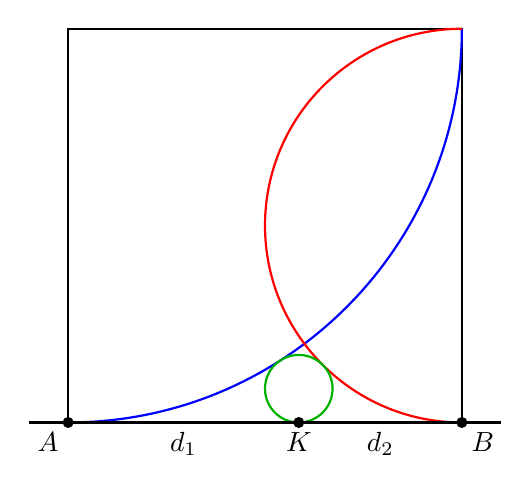
\begin{tikzpicture}[scale=5]
        % Kvadratas
        \draw[thick] (0,0) rectangle (1,1);
        
        % Ketvirtis apskritimo (centras 0,1)
        \draw[thick, blue] (1,1) arc (0:-90:1);
        
        % Pusrutulis (centras 1, 0.5) - išsigaubęs į kairę
        \draw[thick, red] (1,0) arc (270:90:0.5);
        
        % Mažasis apskritimas
        \def\r{0.085786} % (3-2*sqrt(2))/2
        \def\x{0.585786} % 2-sqrt(2)
        \draw[thick, green!70!black] (\x, \r) circle (\r);
        
        % Horizontalioji tangentė
        \draw[thick] (-0.1, 0) -- (1.1, 0);
        
        % Atstumo linijos ir spinduliai (punktyrinės)
        \draw[dashed] (0, 0) -- (\x, 0) node[midway, below] {$d_1$};
        \draw[dashed] (\x, 0) -- (1, 0) node[midway, below] {$d_2$};
        
        % Tangentų taškai
        \fill (0,0) circle (0.4pt);
        \fill (1,0) circle (0.4pt);
        \fill (\x,0) circle (0.4pt);
        
        % Komentarai
        \node[below left] at (0,0) {$A$};
        \node[below] at (\x,0) {$K$};
        \node[below right] at (1,0) {$B$};
    \end{tikzpicture}
    \end{center}

    Mūsų brėžinyje turime:
    \begin{itemize}
        \item Ketvirtis apskritimo atitinka apskritimą (pavadiname $C_1$), kurio spindulys $R_1 = 1$, ir kuris liečia apatinę kvadrato kraštinę taške $A$ (kairiajame apatiniame kampe).
        \item Raudonas pusapskritimis atitinka apskritimą ($C_2$), kurio spindulys $R_2 = 0{,}5$, ir kuris liečia apatinę kraštinę taške $B$ (dešiniajame apatiniame kampe).
        \item Atstumas tarp šių dviejų pradinių lietimosi taškų yra lygus visai kvadrato kraštinei, t.\,y., $AB = 1$.
        \item Mažasis apskritimas (spindulys $r$) liečia abu šiuos apskritimus išorėje ir liečia tą pačią kraštinę taške $K$.
    \end{itemize}
    Pritaikius lemą:
    \begin{itemize}
        \item Atstumas tarp kairiojo kampo ir mažojo apskritimo: $d_1 = 2\sqrt{R_1 r} = 2\sqrt{1 \cdot r} = 2\sqrt{r}$.
        \item Atstumas tarp dešiniojo kampo ir mažojo apskritimo: $d_2 = 2\sqrt{R_2 r} = 2\sqrt{0{,}5 \cdot r} = \sqrt{2r}$.
    \end{itemize}
    Šių dviejų atkarpų suma yra lygi kvadrato kraštinės ilgiui:
    \[ 2\sqrt{r} + \sqrt{2r} = 1. \]
    Išsprendžiame gautą lygtį:
    \[ \sqrt{r}(2 + \sqrt{2}) = 1 \implies \sqrt{r} = \frac{1}{2 + \sqrt{2}}. \]
    Panaikiname iracionalumą vardiklyje (padauginame iš jungtinio $(2 - \sqrt{2})$):
    \[ \sqrt{r} = \frac{2 - \sqrt{2}}{(2 + \sqrt{2})(2 - \sqrt{2})} = \frac{2 - \sqrt{2}}{4 - 2} = \frac{2 - \sqrt{2}}{2}. \]
    Keliame abi puses kvadratu:
    \[ r = \left( \frac{2 - \sqrt{2}}{2} \right)^2 = \frac{4 - 4\sqrt{2} + 2}{4} = \frac{6 - 4\sqrt{2}}{4} = \frac{3 - 2\sqrt{2}}{2}. \]
    
    \textbf{Atsakymas:} $\frac{3 - 2\sqrt{2}}{2}$.

    \vspace{0.3cm}
    \item \textbf{Sprendimas.}
    
    Išskaidykime skaičių pirminiais daugikliais: 
    \[ 1\,000\,000 = 10^6 = 2^6 \cdot 5^6. \]
    Turime rasti tris natūraliuosius daugiklius $x, y, z$, kurių sandauga duoda šią išraišką.
    Kiekvienas daugiklis turi pavidalą $2^{a_i} \cdot 5^{b_i}$, kur indeksas $i \in \{1, 2, 3\}$, o laipsniai $a_i, b_i \ge 0$ yra sveikieji skaičiai.
    Tam, kad sandauga būtų teisinga, visų trijų skaičių laipsnių sumos turi būti lygios 6:
    \begin{align*}
        a_1 + a_2 + a_3 &= 6, \\
        b_1 + b_2 + b_3 &= 6.
    \end{align*}
    
    \textbf{a)} Jei \textbf{atsižvelgiama į tvarką} (daugikliai išdėstyti iš eilės):
    
    Paskaičiuokime, keliais būdais galime gauti sumą 6 iš trijų neneigiamų sveikųjų skaičių. Tai darome sistemingai perrinkdami pirmojo skaičiaus reikšmes:
    \begin{itemize}
        \item Jei $a_1 = 6$, tai $a_2 + a_3 = 0$. Yra \textbf{1} toks būdas (kai $a_2=0, a_3=0$).
        \item Jei $a_1 = 5$, tai $a_2 + a_3 = 1$. Yra \textbf{2} būdai (kai $a_2=1, a_3=0$ arba atvirkščiai).
        \item Jei $a_1 = 4$, tai $a_2 + a_3 = 2$. Yra \textbf{3} būdai.
        \item Jei $a_1 = 3$, tai $a_2 + a_3 = 3$. Yra \textbf{4} būdai.
        \item Jei $a_1 = 2$, tai $a_2 + a_3 = 4$. Yra \textbf{5} būdai.
        \item Jei $a_1 = 1$, tai $a_2 + a_3 = 5$. Yra \textbf{6} būdai.
        \item Jei $a_1 = 0$, tai $a_2 + a_3 = 6$. Yra \textbf{7} būdai.
    \end{itemize}
    Iš viso būdų paskirstyti dvejetų laipsnius $a_1, a_2, a_3$ yra:
    \[ 1 + 2 + 3 + 4 + 5 + 6 + 7 = 28. \]
    Lygiai taip pat, penketų laipsniams $b_1 + b_2 + b_3 = 6$ egzistuoja irgi 28 paskirstymo būdai.
    Kadangi dvejetų ir penketų paskirstymas yra visiškai nepriklausomas, bendras sutvarkytų trejetų skaičius:
    \[ 28 \cdot 28 = 784. \]
    
    \textbf{b)} Jei \textbf{neatsižvelgiama į tvarką} (svarbus tik pats suformuotas skaičių rinkinys):
    
    Padalinkime visus 784 surastus sutvarkytus trejetus į tris grupes pagal tai, kiek rinkinyje yra vienodų daugiklių:
    \begin{itemize}
        \item \textbf{Visi trys daugikliai vienodi ($x = y = z$):} \\
        Jei $x^3 = 1\,000\,000$, tai skaičius gali būti tik $x=100$. Egzistuoja lygiai \textbf{1} toks rinkinys $\{100, 100, 100\}$. Jis sudaro tik 1 sutvarkytą trejetą.
        
        \item \textbf{Lygiai du daugikliai vienodi ($x = y \neq z$):} \\
        Tai reiškia, kad $a_1 = a_2$ ir $b_1 = b_2$.
        Kadangi $a_1 + a_2 + a_3 = 6 \implies 2a_1 + a_3 = 6$, $a_1$ gali įgyti reikšmes $0, 1, 2$ arba $3$ (viso 4 galimybės).
        Taip pat $2b_1 + b_3 = 6$, tad $b_1$ irgi turi 4 galimybes.
        Iš viso galime suformuoti $4 \cdot 4 = 16$ tokių derinių. Viena iš šių kombinacijų ($a_1=2, b_1=2$) mums duos visus 3 vienodus skaičius (kurį aptarėme anksčiau). 
        Likę $16 - 1 = \textbf{15}$ rinkinių turės lygiai 2 vienodus skaičius (pavidalas $\{x, x, z\}$). 
        Kiekvienas toks unikalus rinkinys, sukeičiant skaičius vietomis (pozicijos $(x,x,z), (x,z,x), (z,x,x)$), sukuria po 3 sutvarkytus trejetus, todėl iš viso ši grupė apima $15 \cdot 3 = 45$ sutvarkytus trejetus iš visų 784.
        
        \item \textbf{Visi trys daugikliai skirtingi ($x \neq y \neq z$):} \\
        Atėmę iš visų galimų 784 sutvarkytų trejetų jau aptartus atvejus, gauname sutvarkytus trejetus, sudarytus vien tik iš skirtingų skaičių: 
        \[ 784 - 1 - 45 = 738. \]
        Kadangi trys skirtingi skaičiai gali būti išdėlioti lygiai $6$ skirtingomis tvarkomis ($3 \cdot 2 \cdot 1 = 6$), tai unikalių nesutvarkytų rinkinių šioje grupėje yra:
        \[ \frac{738}{6}  = 123. \]
    \end{itemize}
    
    Galutinis nesutvarkytų trejetų (rinkinių) skaičius yra:
    \[ 1 \text{ (visi vienodi)} + 15 \text{ (du vienodi)} + 123 \text{ (visi skirtingi)} = 139. \]
    
    \textbf{Atsakymas:} a) 784; \quad b) 139.
\end{enumerate}

\end{document}